\documentclass[11pt,a4paper]{article}
\usepackage[utf8]{inputenc}
\usepackage[T1]{fontenc}
\usepackage[english,french]{babel}
\usepackage{amsmath, amsfonts, amssymb}
\usepackage{graphicx}
\usepackage{geometry}
\usepackage{hyperref}
\usepackage{xcolor}
\usepackage{listings}
\usepackage{float}
\usepackage{booktabs}
\usepackage{enumitem}

\geometry{
    top=2.5cm,
    bottom=2.5cm,
    left=2.5cm,
    right=2.5cm
}

% Code listing settings
\definecolor{codegreen}{rgb}{0,0.6,0}
\definecolor{codegray}{rgb}{0.5,0.5,0.5}
\definecolor{codepurple}{rgb}{0.58,0,0.82}
\definecolor{backcolour}{rgb}{0.95,0.95,0.92}

\lstdefinestyle{mystyle}{
    backgroundcolor=\color{backcolour},   
    commentstyle=\color{codegreen},
    keywordstyle=\color{magenta},
    numberstyle=\tiny\color{codegray},
    stringstyle=\color{codepurple},
    basicstyle=\ttfamily\footnotesize,
    breakatwhitespace=false,         
    breaklines=true,                 
    captionpos=b,                    
    keepspaces=true,                 
    numbers=left,                    
    numbersep=5pt,                  
    showspaces=false,                
    showstringspaces=false,
    showtabs=false,                  
    tabsize=2
}
\lstset{style=mystyle}

\title{\textbf{Fuzzy Logic \& Explainable AI (XAI)}\\ \Large Summary and Exam Preparation}
\author{}
\date{}

\begin{document}

\maketitle

\tableofcontents
\newpage

\section{Fuzzy Logic}

\subsection{Classic Sets vs. Fuzzy Sets}
\begin{itemize}
    \item \textbf{Classic Sets (Ensembles classiques):} In traditional logic, an item completely belongs to a group (a value of 1) or it doesn't belong at all (a value of 0).
    \item \textbf{Fuzzy Sets (Ensembles flous):} Fuzzy logic allows for \textit{partial} belonging. An item's membership can be any value in the interval $[0, 1]$.
\end{itemize}

\subsection{Basic Characteristics of Fuzzy Sets}
Let $A$ be a fuzzy set defined on an universe $X$, with a membership function $\mu_A(x)$.
\begin{itemize}
    \item \textbf{Le support (Support):} Items that belong to the set even a tiny bit ($\mu_A(x) > 0$).
    \[ \text{supp}(A) = \{x \in X \mid \mu_A(x) > 0\} \]
    
    \item \textbf{Le noyau (Kernel):} Items that perfectly and completely belong to the set.
    \[ \text{Noyau}(A) = \{x \in X \mid \mu_A(x) = 1\} \]
    
    \item \textbf{La hauteur (Height):} The highest possible membership score in the set.
    \[ H(A) = \sup_{x \in X} \mu_A(x) \]
    
    \item \textbf{$\alpha$-Coupe (Alpha-cut):} A filter keeping only items with a membership score above a threshold $\alpha$.
    \[ A_\alpha = \{x \in X \mid \mu_A(x) \geq \alpha\} \]
    
    \item \textbf{Point de croisement (Crossover point):} The point where the membership score is exactly $0.5$.
    
    \item \textbf{Ensembles flous normalisés (Normalized fuzzy sets):} A set is normalized if at least one item reaches a perfect score of 1.
    \[ A \text{ est normalisé } \iff \exists x \in X, \mu_A(x) = 1 \]
    
    \item \textbf{Convexité:} Un ensemble flou est convexe si et seulement si ses $\alpha$-coupes sont convexes.
\end{itemize}
\vspace{0.5cm}
\textit{Note: Reference figures fig1.1.png and fig1.2.png illustrate normalization and convexity.}

\subsection{The Linguistic Variable}
Fuzzy logic computes using everyday words instead of exact numbers to mimic human reasoning.
\begin{itemize}
    \item \textbf{L'univers du discours (Universe of discourse):} The complete range of possible values for a variable.
    \item \textbf{Valeurs linguistiques (Linguistic values):} Descriptive words used for parts of that range (e.g., ``cold'', ``young'').
    \item \textbf{Fonction d'appartenance (Membership function):} Mathematical shapes mapping these words to numbers (e.g., Triangular, Gaussian, Trapezoidal).
\end{itemize}
\textit{Note: Reference figure fig1.3.png illustrates linguistic variables.}

\subsection{Fuzzy Logic Operators (Lotfi A. Zadeh, 1973)}
When combining fuzzy sets, specific mathematical rules introduced by Lotfi A. Zadeh in 1973 are applied:
\begin{itemize}
    \item \textbf{ET logique (Logical AND):} Represents intersection (takes the minimum).
    \[ \mu_{A \cap B}(x) = \min(\mu_A(x), \mu_B(x)) \]
    \begin{center}
        \begin{tabular}{|c|c|c|}
            \hline
            A & B & A AND B ($\cap$) \\ \hline
            0 & 0 & 0 \\ \hline
            0 & 1 & 0 \\ \hline
            1 & 0 & 0 \\ \hline
            1 & 1 & 1 \\ \hline
        \end{tabular}
    \end{center}
    
    \item \textbf{OU logique (Logical OR):} Represents union (takes the maximum).
    \[ \mu_{A \cup B}(x) = \max(\mu_A(x), \mu_B(x)) \]
    \begin{center}
        \begin{tabular}{|c|c|c|}
            \hline
            A & B & A OR B ($\cup$) \\ \hline
            0 & 0 & 0 \\ \hline
            0 & 1 & 1 \\ \hline
            1 & 0 & 1 \\ \hline
            1 & 1 & 1 \\ \hline
        \end{tabular}
    \end{center}
    
    \item \textbf{NON logique (Logical NOT):} Represents the opposite (complement).
    \[ \mu_{\bar{A}}(x) = 1 - \mu_A(x) \]
    \begin{center}
        \begin{tabular}{|c|c|}
            \hline
            A & NOT A ($\neg$) \\ \hline
            0 & 1 \\ \hline
            1 & 0 \\ \hline
        \end{tabular}
    \end{center}
\end{itemize}
\textit{Note: Reference figures fig1.4.png, fig1.5.png, and fig1.6.png.}

\newpage
\section{Inference Systems: Classic vs. Fuzzy}

\subsection{Classic Inference Systems}
Uses strict Boolean logic (0=False, 1=True) to deduce conclusions.
\begin{itemize}
    \item \textbf{Components:}
    \begin{itemize}
        \item \textbf{Base de connaissances (Knowledge Base):} Contains the \textit{Database} (known facts, e.g., Temp=15) and \textit{Rule Base} (strict IF-THEN rules).
        \item \textbf{Moteur d'inférence (Inference Engine):} Mechanism that applies rules to data.
        \item \textbf{Interface utilisateur:} User interaction component.
    \end{itemize}
    \item \textbf{Inference Methods:}
    \begin{itemize}
        \item \textit{Forward Chaining (Chaînage avant):} Facts $\rightarrow$ Rules $\rightarrow$ Conclusion.
        \item \textit{Backward Chaining (Chaînage arrière):} Goal/Conclusion $\rightarrow$ Rules $\rightarrow$ Verify facts.
    \end{itemize}
    \item \textbf{Pros \& Cons:} Simple, fast, but cannot handle uncertainty/vague concepts and has abrupt boundaries.
\end{itemize}

\subsection{Fuzzy Inference Systems (FIS)}
Handles uncertainty using linguistic variables. Membership degrees can be any value in $[0, 1]$.
\begin{itemize}
    \item \textbf{Formal Definition:} Defined by $(X, Y, F, R, M)$, where $X, Y$ are input/output variables, $F$ are membership functions, $R$ are fuzzy rules, and $M$ is the inference method.
    \item \textbf{The Steps:}
    \begin{enumerate}
        \item \textbf{Fuzzification:} Converting a precise number into a membership degree (e.g., Temp=25 $\rightarrow \mu_{froid}(25)=0.2$).
        \item \textbf{Inference:} Applying linguistic rules (e.g., IF Temp is Cold THEN Fan is Slow).
        \item \textbf{Defuzzification:} Converting the final fuzzy result back into a precise, usable number.
    \end{enumerate}
\end{itemize}
\textit{Note: Reference figures fig2.1 and fig2.2.}

\subsection{Fuzzy Inference Models}
\begin{itemize}
    \item \textbf{Le modèle Mamdani:} Most commonly used. The conclusion of each rule is a fuzzy set. Defuzzification uses the weighted average of the centers:
    \[ z = \frac{\sum (w_i \cdot C_i)}{\sum w_i} \]
    (where $w_i$ is the rule's weight/activation degree and $C_i$ is the center of the output shape).
    
    \item \textbf{Le modèle Sugeno:} The conclusion is a strict mathematical function, great for calculations and optimization.
    \[ z = \frac{\sum (w_i \cdot z_i)}{\sum w_i} \]
    (where $z_i$ is a strict mathematical equation instead of a shape).
    
    \item \textbf{Modèle Tsukamoto:} Output sets must be strictly increasing or decreasing (monotonic). Find the specific output $z_i$ where membership equals activation degree $\alpha_i$:
    \[ z = \frac{\sum (\alpha_i \cdot z_i)}{\sum \alpha_i} \]
\end{itemize}

\newpage
\section{Fuzzy Clustering (FCM)}

\subsection{Classic (Hard) Clustering Review}
\begin{itemize}
    \item \textbf{Definition:} Unsupervised learning grouping data based on similarity (minimize intra-cluster distance, maximize inter-cluster distance).
    \item \textbf{Hard Clustering:} A point belongs to exactly one cluster. $u_{ij} \in \{0, 1\}$.
    \item \textbf{K-means Objective Function:} $J = \sum_{i=1}^n \sum_{j=1}^c ||x_i - c_j||^2$.
    \item \textbf{Limitations:} Abrupt assignments, information loss, and sensitivity to noise.
\end{itemize}

\subsection{Fuzzy Clustering Mathematical Formalism}
Fixes limitations of hard clustering: a point can belong to multiple clusters simultaneously.
\begin{itemize}
    \item \textbf{Constraints:}
    \[ 0 \leq u_{ij} \leq 1 \quad \text{and} \quad \sum_{j=1}^{c} u_{ij} = 1 \]
    \item \textbf{FCM Objective Function:} Minimize the error:
    \[ J_m = \sum_{i=1}^{n}\sum_{j=1}^{c} u_{ij}^m ||x_i - c_j||^2 \]
    where $m$ is the fuzziness coefficient.
\end{itemize}

\subsection{FCM Algorithm Steps}
\begin{enumerate}
    \item \textbf{Initialization:} Choose number of clusters $c$ and initialize membership matrix $U$.
    \item \textbf{Calculate Cluster Centers ($c_j$):} Weighted average of points.
    \[ c_j = \frac{\sum_{i=1}^{n} u_{ij}^m x_i}{\sum_{i=1}^{n} u_{ij}^m} \]
    \item \textbf{Update Memberships ($u_{ij}$):}
    \[ u_{ij} = \frac{1}{\sum_{k=1}^{c} \left( \frac{||x_i - c_j||}{||x_i - c_k||} \right)^{\frac{2}{m-1}}} \]
    \item \textbf{Stopping Criteria:} Repeat steps 2 and 3 until $||U_{new} - U|| < \epsilon$.
\end{enumerate}

\subsection{FCM Python Implementation}
\begin{lstlisting}[language=Python, caption=Fuzzy C-Means Algorithm Implementation]
import numpy as np

# 1. DATA INITIALIZATION
X = np.array([1, 2, 5, 8], dtype=float) # Note: Example data points
n = len(X)
c = 2 # Number of clusters
m = 2 # Fuzziness coefficient
epsilon = 0.1 # Stopping criteria
max_iter = 100 

# Initial membership matrix U
U = np.array([
    [0.8, 0.2],
    [0.7, 0.3],
    [0.3, 0.7],
    [0.2, 0.8]
], dtype=float)

# 2. MATH FUNCTIONS
def calcul_centres(X, U, m):
    um = U ** m
    # Weighted average
    centres = (um.T @ X) / np.sum(um.T, axis=1) 
    return centres

def update_U(X, centres, m):
    n, c = len(X), len(centres)
    U_new = np.zeros((n, c))
    for i in range(n):
        for j in range(c):
            somme = 0
            for k in range(c):
                d1 = abs(X[i] - centres[j])
                d2 = abs(X[i] - centres[k])
                if d2 == 0:
                    d2 = 1e-6 # Avoid division by zero
                somme += (d1 / d2) ** (2 / (m - 1))
            U_new[i, j] = 1 / somme
    return U_new

# 3. ALGORITHM LOOP
iteration = 0
while iteration < max_iter:
    iteration += 1
    centres = calcul_centres(X, U, m) # Step A
    U_new = update_U(X, centres, m)   # Step B
    
    # Step C: Convergence Test
    if np.linalg.norm(U_new - U) < epsilon:
        break
    U = U_new
\end{lstlisting}

\newpage
\section{Adaptive Neuro-Fuzzy Inference System (ANFIS)}

\subsection{Why ANFIS?}
\begin{itemize}
    \item \textbf{ANN (Artificial Neural Networks):} Powerful but act as an opaque "black box" (cannot explain decisions).
    \item \textbf{Fuzzy Logic:} Highly interpretable but requires manual rule creation.
    \item \textbf{ANFIS:} Combines both! It learns parameters automatically from data (like ANN) while generating clear, interpretable IF-THEN rules (like Fuzzy).
\end{itemize}

\subsection{Definition \& Architecture}
A hybrid model that uses Sugeno fuzzy rules structured inside a neural network architecture, allowing it to automatically learn and adjust its parameters.
\\
\textbf{The 5 Layers Architecture:}
\begin{enumerate}
    \item \textbf{Layer 1 - Fuzzification (Fonctions d'appartenance):} Calculates membership degrees (e.g., using Gaussian functions).
    \item \textbf{Layer 2 - Rule Activation (Calcul des poids):} Multiplies inputs to find the activation strength of the rule.
    \item \textbf{Layer 3 - Normalization:} Calculates the relative weight of the rule compared to all others.
    \item \textbf{Layer 4 - Rule Output (Conséquent Sugeno):} Applies the mathematical Sugeno function.
    \item \textbf{Layer 5 - Final Output (Défuzzification):} Calculates the final global output.
\end{enumerate}

\subsection{Comparison: ANFIS vs. ANN}
\begin{itemize}
    \item \textbf{ANN:} "I predict, but I cannot explain" (Black box).
    \item \textbf{ANFIS:} "I predict AND I explain using rules" (Interpretable).
\end{itemize}

\subsection{Pros and Cons}
\begin{itemize}
    \item \textbf{Pros:} Interpretable, automatic hybrid learning, highly precise.
    \item \textbf{Cons:} Computationally expensive, high number of parameters, sensitive to data.
\end{itemize}

\subsection{Real-World Applications}
\begin{itemize}
    \item \textbf{Credit Risk Example:} "SI revenu est faible ET dette est élevée ALORS crédit = refusé".
    \item \textbf{Other Applications:} Medical diagnosis, finance, predictive maintenance, smart grids, robotics, Explainable AI (XAI).
\end{itemize}

\newpage
\section{Fuzzy Quantifiers}

\subsection{Why use them?}
\begin{itemize}
    \item \textbf{Why use them? (Pourquoi les utiliser ?):} Classic rules (like "IF CPU is high") are too rigid. Quantifiers (like "IF most indicators are high") make the rules much more natural, flexible, and interpretable.
    \item \textbf{Formal Definition (Définition formelle):} A fuzzy quantifier is a mathematical function that takes a satisfied proportion ($p$) and converts it into a degree of truth ($Q(p)$).
    \[ Q: [0, 1] \rightarrow [0, 1] \]
    \item \textbf{Pros \& Cons (Avantages et Inconvénients):}
    \begin{itemize}
        \item \textit{Pros:} Uses natural human language, improves explainability, and handles vague concepts perfectly.
        \item \textit{Cons:} The choice of the function is highly subjective and can be difficult to calibrate.
    \end{itemize}
    \item \textbf{Mathematical Example (Exemple mathématique):} To calculate the exact degree of truth for the word "most" (\textit{la plupart}):
    \[
    Q_{\text{most}}(p) = 
    \begin{cases} 
      0 & \text{for } p < 0.5 \\
      2p - 1 & \text{for } 0.5 \leq p \leq 1 
    \end{cases}
    \]
    \textit{Interpretation:} If less than 50\% of conditions are met, "most" is 0\% true. Once past 50\%, the truth degree scales up progressively until 100\% truth at $p=1$.
\end{itemize}

\subsection{Types of Fuzzy Quantifiers}
\begin{itemize}
    \item \textbf{Monotonic Quantifiers (Quantificateurs monotones):} Functions that only go in one direction (strictly increasing like "a lot" or strictly decreasing like "few").
    \begin{itemize}
        \item \textit{Property:} If $x_1 \leq x_2$, then $Q(x_1) \leq Q(x_2)$.
        \item \textit{Pros/Cons:} Logically coherent, but cannot cover specific target concepts like "around 5".
    \end{itemize}
    \item \textbf{Non-monotonic Quantifiers (Quantificateurs non monotones):} Functions centered on a specific target value, using triangular or Gaussian shapes (e.g., "about 5", "almost half").
    \begin{itemize}
        \item \textit{Pros/Cons:} Great for precise concepts, but more complex and less stable.
    \end{itemize}
    \item \textbf{Regular Quantifiers (Quantificateurs réguliers de Zadeh):} These must strictly start at zero and end at exactly one.
    \begin{itemize}
        \item \textit{Property:} $Q(0) = 0$ and $Q(1) = 1$.
        \item \textit{Examples:} "most", "a lot".
        \item \textit{Pros/Cons:} Perfectly compatible with standard fuzzy logic, but limited to proportional cases.
    \end{itemize}
    \item \textbf{Non-regular Quantifiers (Quantificateurs non réguliers):} These do not respect Zadeh's strict boundaries.
    \begin{itemize}
        \item \textit{Examples:} "about 5", "exactly 3".
        \item \textit{Pros/Cons:} Very flexible for real-world situations, but less compatible with standard mathematical models.
    \end{itemize}
    \item \textbf{Linguistic Quantifiers (Quantificateurs linguistiques flous):} Natural language expressions modeled directly by fuzzy functions (e.g., "few", "enough").
    \begin{itemize}
        \item \textit{Pros/Cons:} Extremely natural for the user and expert systems, but highly subjective and require careful calibration.
    \end{itemize}
\end{itemize}

\subsection{Integration in Fuzzy Rules (Intégration des quantificateurs flous dans les règles floues)}
\begin{itemize}
    \item \textbf{The Problem with Classic Rules:} Without quantifiers, a standard fuzzy rule looks like: \textit{IF Temperature is hot THEN Fan is fast}. While functional, this approach is often considered too raw, rigid, and lacking nuance to model complex scenarios.
    \item \textbf{Integration of Quantifiers:} Adding quantifiers enriches these rules to make them more nuanced and interpretable. For example:
    \begin{itemize}
        \item R1: \textit{SI Température est très chaude ALORS Ventilateur est très rapide.}
        \item R2: \textit{SI Température est moyennement chaude ALORS Ventilateur est moyen.}
        \item R3: \textit{SI Température est peu chaude ALORS Ventilateur est lent.}
    \end{itemize}
    \item \textbf{Effect of Modifiers:} On a logical level, each word mathematically modifies the raw information:
    \begin{itemize}
        \item "Très" (Very) reinforces the condition.
        \item "Moyennement" (Moderately) softens the condition.
        \item "Peu" (Little) reverses or reduces the condition.
    \end{itemize}
    \item \textbf{Added Value (Conclusion):} Using quantifiers transforms simple rules into rich linguistic expressions. This brings very strong explainability to the system, greater flexibility, and reproduces human reasoning much more faithfully.
\end{itemize}


\section{Fuzzy Decision Trees}

\subsection{Introduction \& Review (Arbres de Décision Classiques)}
\begin{itemize}
    \item \textbf{Classic Trees (Arbres classiques):} Supervised learning models making hierarchical decisions via rules. They consist of a root node, branches, and leaves, where each node applies a strict, precise binary test (e.g., Age > 30).
\begin{verbatim}
        Age > 30 ?
        /        \
      Oui        Non
      /            \
Revenu eleve ?    Refus
    /      \
  Oui      Non
Accepte   Refus
\end{verbatim}
    \item \textbf{Fuzzy Decision Trees (Arbres de Décision Flous):} Extend classic trees using fuzzy logic to handle uncertainty and imprecision. A single data point can belong partially to multiple classes.
    \item \textbf{Construction of a Classic Tree:} Uses algorithms like ID3, C4.5, and CART to find the best attributes to separate the data based on calculation criteria:
    \begin{itemize}
        \item \textbf{Entropy (Entropie):} Calculates uncertainty.
        \[ H(S) = - \sum_{i=1}^{n} p_i \log_2(p_i) \]
        \item \textbf{Information Gain (Gain d'information):} Calculates the reduction in uncertainty to pick the best attribute.
        \[ Gain(S,A) = H(S) - \sum_{v \in Values(A)} \left( \frac{|S_v|}{|S|} \right) H(S_v) \]
    \end{itemize}
\end{itemize}
\begin{figure}[H]
    \centering
    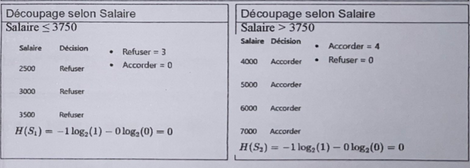
\includegraphics[width=0.7\textwidth]{figs/6/fig6.1.png}
    \caption{Example of a classic decision tree.}
\end{figure}

\subsection{Why Use a Fuzzy Decision Tree? (Limites de l'arbre classique)}
Classic trees have several limitations:
\begin{itemize}
    \item \textbf{Strict Boundaries (Frontières de décision brutales):} Rigid cutoffs are not realistic (e.g., a tiny change leads to opposite decisions).
    \item \textbf{No Linguistic Terms (Absence de notion linguistique):} They manipulate exact numbers instead of human concepts like "salaire faible".
    \item \textbf{Poor Uncertainty Handling (Mauvaise gestion de l'incertitude):} Highly unstable to small data variations.
    \item \textbf{Rule Explosion \& Overfitting (Surapprentissage):} Deep trees memorize training data but fail on new clients.
\end{itemize}
\textbf{The Fuzzy Solution:} Fuzzy trees replace strict bounds with membership degrees, making decisions progressive instead of binary.

\subsection{Construction of a Fuzzy Decision Tree}
The goal is to build the tree using fuzzy membership degrees, calculate fuzzy entropies, and generate fuzzy rules.
\begin{itemize}
    \item \textbf{Fuzzy Sets (Ensembles flous):} Instead of a strict boundary, variables are divided into fuzzy sets like "Faible", "Moyen", and "Élevé".
    \item \textbf{Fuzzy Entropy (Entropie Floue):} Similar to classic entropy, but uses fuzzy probabilities. To find the probability, you sum the membership degrees for each class instead of counting whole units.
\end{itemize}

\subsection{Rule Generation (Génération des règles)}
\begin{itemize}
    \item \textbf{Fuzzy Weights (Poids flous des ensembles):} The weight of each fuzzy branch is calculated by summing the membership degrees.
    \item \textbf{Fuzzy Information Gain (Gain d'Information Flou):} Determines which attribute to place at the top of the tree.
\begin{verbatim}
         Salaire
       /    |    \
  Faible  Moyen  Eleve
    |       |      |
 Refuser  Mixte  Accorder
\end{verbatim}
    \item \textbf{Rule Generation Principle:} A rule is created by taking the fuzzified values, selecting the dominant class, and translating the path into natural linguistic terms.
\end{itemize}
\textbf{Examples of generated rules:}
\begin{itemize}
    \item \textit{Règle 1:} IF Salary is Low AND Debt is High THEN Decision = Refuse
    \item \textit{Règle 2:} IF Salary is Medium AND Age is Young AND Debt is Medium THEN Decision = Accept
    \item \textit{Règle 3:} IF Salary is High AND Age is Medium AND Debt is Low THEN Decision = Accept
\end{itemize}

\subsection{Conclusion (Arbres flous)}
\begin{itemize}
    \item \textbf{Main Advantages:} Better uncertainty management, progressive decisions, greater robustness, and rules that map closely to natural human reasoning.
    \item \textbf{Applications:} Expert systems, finance, medicine, and general decision support.
\end{itemize}

\end{document}
